\chapter{Experimental validation} % (fold)
\label{cha:experimental_validation}
    In this chapter I'll show the results of the execution of the two versions, standard and fastflow, of the
    program implementing the watermarking project. As explained in chapter \ref{cha:performance_modeling}, I've
    considered the most known measures from the parallel/distributed computing point of view. Figure
    \ref{fig:performances} represents the progress of every measure compared to the parallelism degree that, for
    the standard program, ranges from $0$ to $10$, and, for the fastflow versions, ranges from $1$ to $10$.
    \section{Completion time} % (fold)
    \label{sec:completion_time}

    % section completion_time (end)
    \section{Speedup} % (fold)
    \label{sec:speedup}

    % section speedup (end)
    \section{Scalability} % (fold)
    \label{sec:scalability}

    % section scalability (end)
    \section{Efficiency} % (fold)
    \label{sec:efficiency}

    % section efficiency (end)
    \begin{figure}
        \centering
        \begin{subfigure}{0.33\textwidth}
            \resizebox{\textwidth}{!}{
                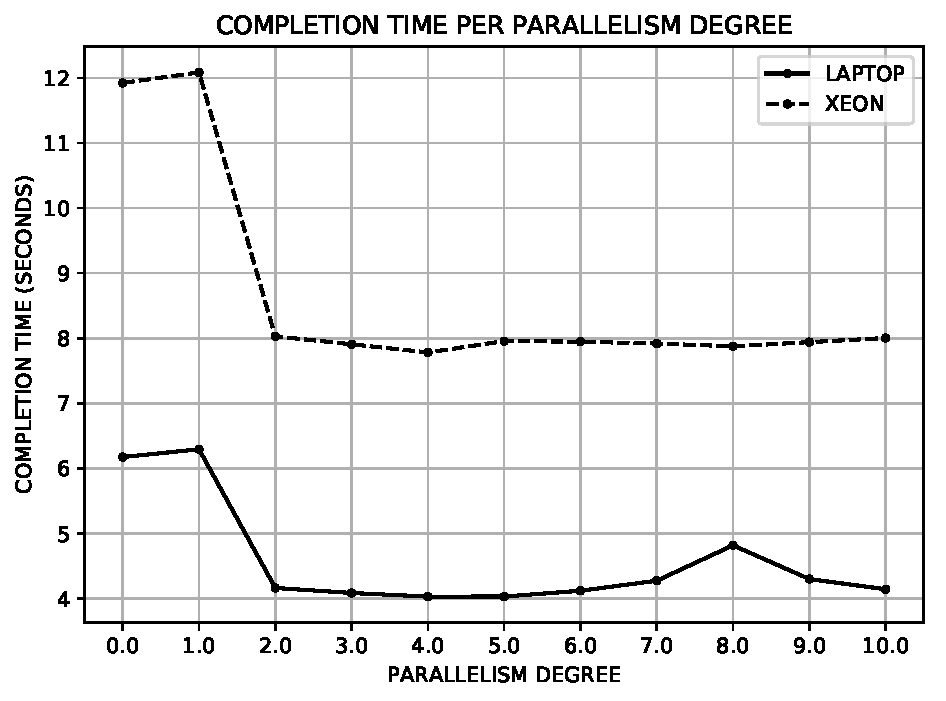
\includegraphics{imgs/completion_time_standard.pdf}
            }
            \caption{Standard}
            \label{fig:completion_time_standard}
        \end{subfigure}
        \begin{subfigure}{0.33\textwidth}
            \resizebox{\textwidth}{!}{
                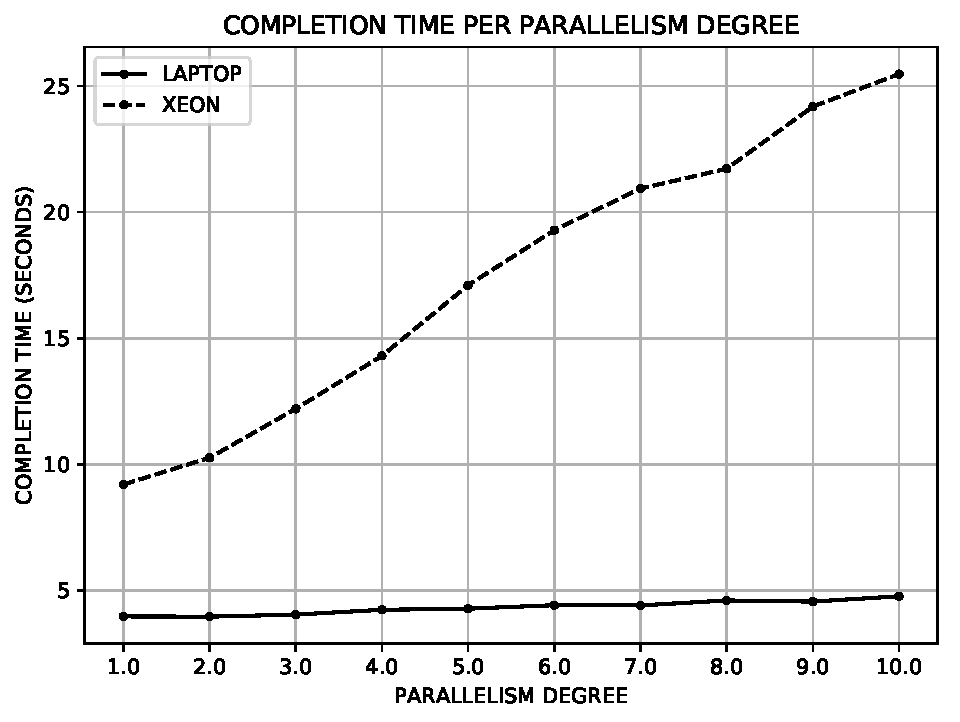
\includegraphics{imgs/completion_time_fastflow.pdf}
            }
            \caption{Fastflow}
            \label{fig:completion_time_fastflow}
        \end{subfigure}
        \begin{subfigure}{0.33\textwidth}
            \resizebox{\textwidth}{!}{
                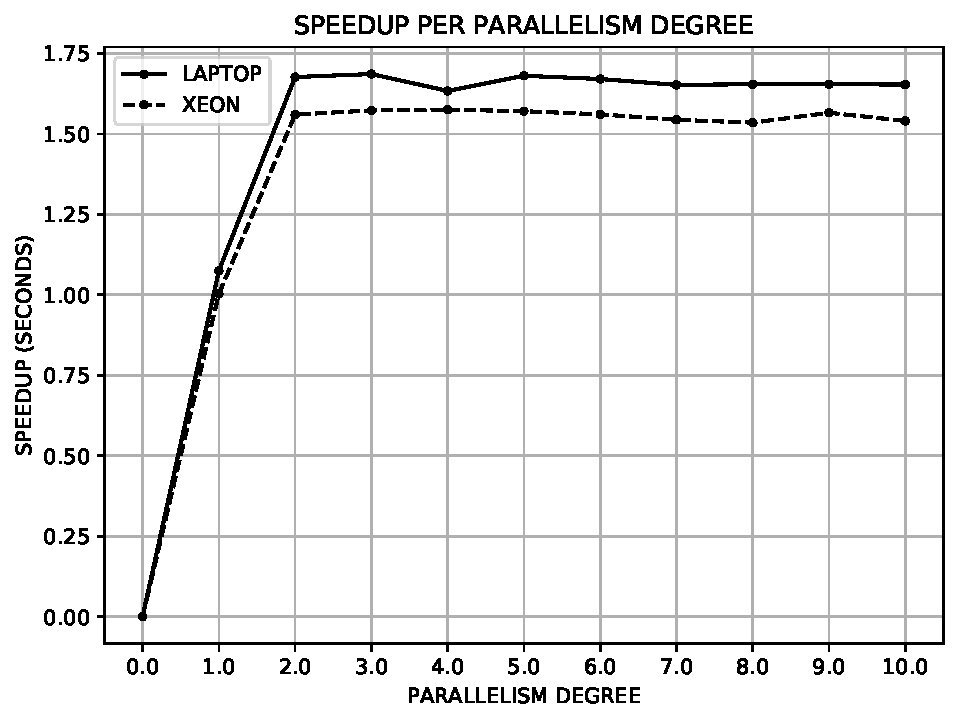
\includegraphics{imgs/speedup_standard.pdf}
            }
            \caption{Standard}
            \label{fig:speedup_standard}
        \end{subfigure}
        \begin{subfigure}{0.33\textwidth}
            \resizebox{\textwidth}{!}{
                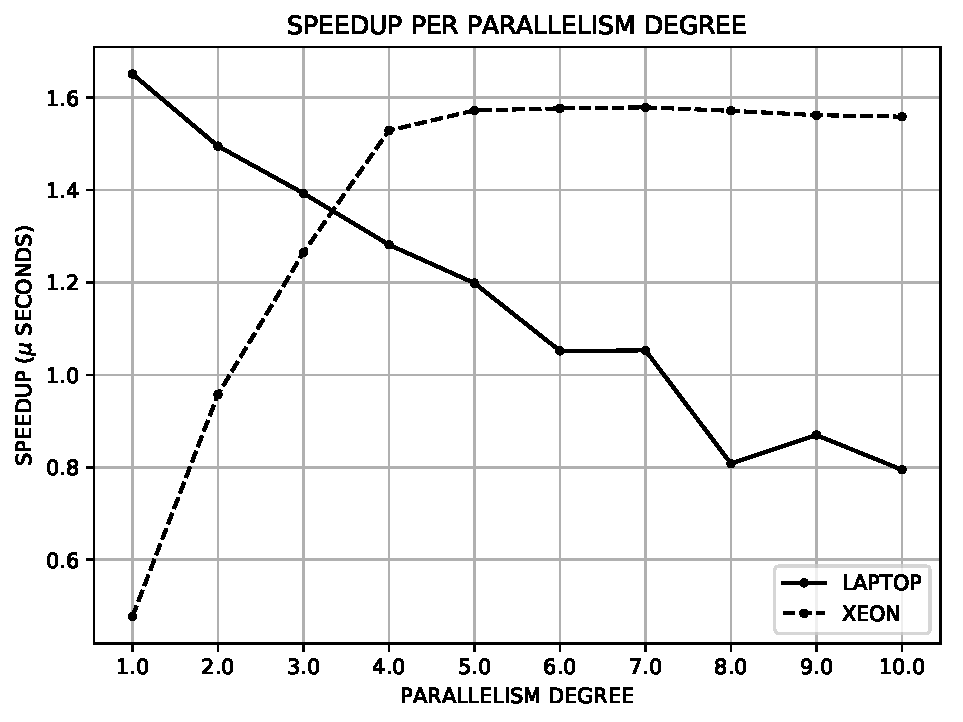
\includegraphics{imgs/speedup_fastflow.pdf}
            }
            \caption{Fastflow}
            \label{fig:speedup_fastflow}
        \end{subfigure}
        \begin{subfigure}{0.33\textwidth}
            \resizebox{\textwidth}{!}{
                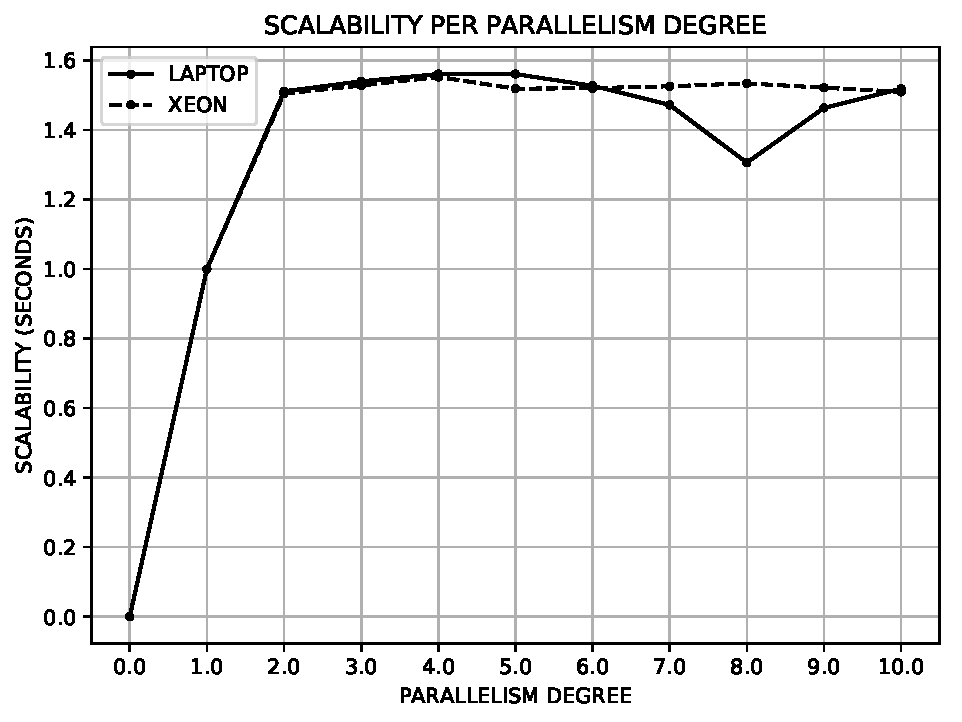
\includegraphics{imgs/scalability_standard.pdf}
            }
            \caption{Standard}
            \label{fig:scalability_standard}
        \end{subfigure}
        \begin{subfigure}{0.33\textwidth}
            \resizebox{\textwidth}{!}{
                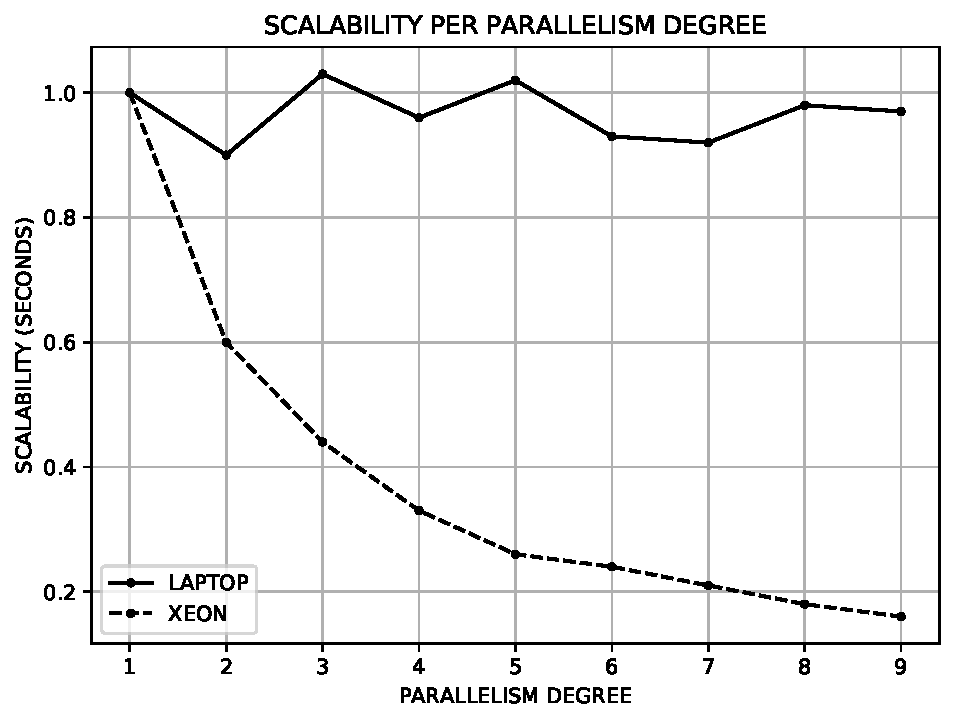
\includegraphics{imgs/scalability_fastflow.pdf}
            }
            \caption{Fastflow}
            \label{fig:scalability_fastflow}
        \end{subfigure}
        \begin{subfigure}{0.33\textwidth}
            \resizebox{\textwidth}{!}{
                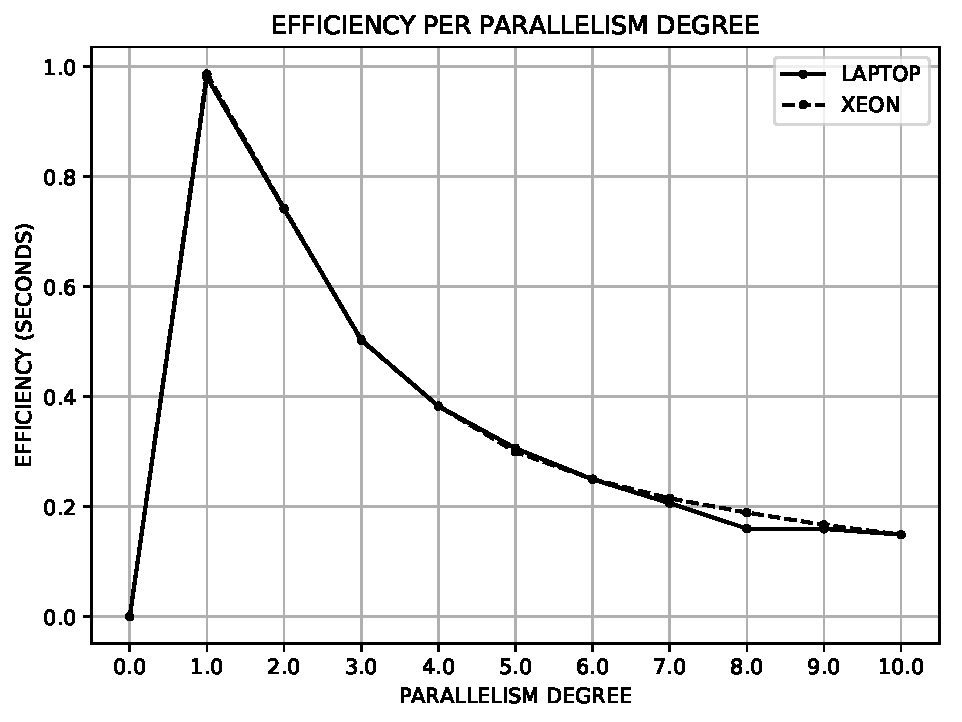
\includegraphics{imgs/efficiency_standard.pdf}
            }
            \caption{Standard}
            \label{fig:efficiency_standard}
        \end{subfigure}
        \begin{subfigure}{0.33\textwidth}
            \resizebox{\textwidth}{!}{
                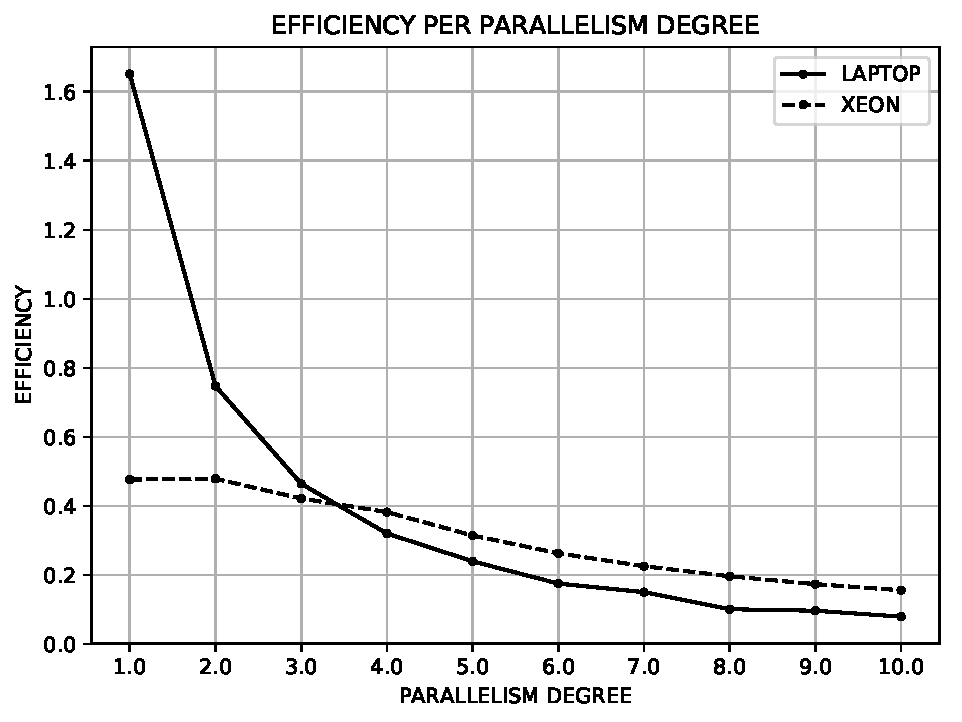
\includegraphics{imgs/efficiency_fastflow.pdf}
            }
            \caption{Fastflow}
            \label{fig:efficiency_fastflow}
        \end{subfigure}
        \caption{}
        \label{fig:performances}
    \end{figure}
    \newpage
    \pagenumbering{Roman}
    \setcounter{page}{2}
% chapter experimental_validation (end)
